%%%%%%%%%%%%%%%%%%%%%%%%%%%%%%%%%%%%%%%%%%%%%%%%%%%
%
%  New template code for TAMU Theses and Dissertations starting Spring 2021.  
%
%
%  Author: Thesis Office
%  
%  Last Updated: 1/13/2021
%
%%%%%%%%%%%%%%%%%%%%%%%%%%%%%%%%%%%%%%%%%%%%%%%%%%%

%%%%%%%%%%%%%%%%%%%%%%%%%%%%%%%%%%%%%%%%%%%%%%%%%%%%%%%%%%%%%%%%%%%%%%%
%%%                           SECTION II
%%%%%%%%%%%%%%%%%%%%%%%%%%%%%%%%%%%%%%%%%%%%%%%%%%%%%%%%%%%%%%%%%%%%%%


\chapter{\MakeUppercase{Literature Review}}
\label{cha:literature-review}

A review of the literature surrounding information quality research within market monitoring units shows that there is a legitimate gap in how value is being derived from information assets. This gap is highlighted by several major issues (introduced in Chapter \ref{cha:Introduction} and discussed in this literature review), including: 

\begin{enumerate}
    \item{An aging workforce in the electric utilities industry that is reaching the tipping point for replacement}
    \item{A disruption of traditional energy market design due to advances in technology and the regulatory landscape}
    \item{A lack of focus on data and information quality research within the electric utilities industry}
\end{enumerate}

\noindent These issues represent a unique opportunity to yield important value from the data assets both generated and used by actors in the market monitoring sphere. The researcher will discuss each of these issues in the context of relevant literature,
\footnote{Appendix \ref{appendix:B} contains a listing of different search phrases used for finding relevant research included in this literature review.}
and then introduce other relevant research that indicates how this design science project has the potential to improve these issues in the market monitoring landscape.

\section{Business Landscape}
\subsection{An Aging Workforce}

Many technical workforces are seeing a similar problem of an aging workforce; trained professionals are reaching retirement age at a rate faster than that of replacement. A 2006 study showed that the largest staff segment, of a surveyed group of energy professionals, is at (or beyond) retirement age. This same study cited "retirements, restructuring, and technology changes" as being the primary drivers of staff leaving the energy profession \cite{raysnyder}. Such a problem impacts market monitoring as well.

MMUs (as previously discussed) were cemented into operation by the US federal government, not long before that same 2006 study. An energy research lab at UC Berkeley shows that staffing across market monitors is relatively low compared to other organizations in the industry. According to Goldman, Lesieutre, and Bartholomew, all operational market monitoring groups in the US had fewer than 20 FTEs (each) in employ by 2004 \cite{goldman}.

While these numbers appear low in comparison to other organizations with energy industry staff \footnote{As of Q1 2025, Southwest Power Pool employs over 800 FTEs (including their internal market monitoring staff).}
, this study declares that budgets and headcount (at that time) increased significantly for market monitoring work. As such, this shows a trend of growing demand for market monitoring staff in a workforce that, holistically, employs many individuals on (or beyond) the horizon of retirement. One claim to helping combat this “brain drain” problem is a technology framework that “facilitates knowledge retention” \cite{raysnyder}, including systems (supported by an IT organization) that capture necessary processual knowledge.

\subsection{Formation of Market Monitoring Units}

Market monitoring units were formed in response to sweeping changes in how US corporations are now regulated. The fall of Enron Corporation gave way to the rise of the Sarbanes-Oxley Act of 2002, which issued stringent financial reporting and auditing requirements for all publicly traded companies. The Energy Policy Act of 2005, several years later, gave more authority for regulatory bodies to pursue cases of market manipulation and marketplace gaming. In addition, the act also elevated the definition of market manipulation for energy market participants.

To paraphrase the legislation, "it shall be unlawful for any entity... to use or employ, in connection with the purchase or sale of electric energy or the purchase or sale of transmission services subject to the jurisdiction of the Commission, any manipulative or deceptive device or contrivance..., in contravention of such rules and regulations as the Commission may prescribe as necessary or appropriate in the public interest or for the protection of electric ratepayers" \cite{epa2005}. In addition to electricity markets, natural gas markets also saw an increase in regulatory activity.

Coming into the current decade (2020's), we now see a slew of new external factors that affect the energy industry (and by extension, also affect the market monitoring domain) including:

\begin{itemize}
    \item{A global transition away from the use of fossil fuels in energy production}
    \item{Increased penalties for excess greenhouse gas emissions}
    \item{Developments in energy storage}
    \item{Enrollment of large energy consumers as demand response resources}
    \item{Renewable energy technology}
\end{itemize} 

Each of these factors have an effect on the energy market landscape \cite{bichler}. In response, market monitors must develop strategies to observe these new market dynamics. These industry changes add to the data entropy in which market monitoring analysts operate. New standards for greenhouse gas emissions give way for new tactics that market participants can use as excuses for what is currently identified as manipulative behavior \footnote{For example, a gas turbine generator that uneconomically produces power in a market interval can claim that they had to underproduce as part of curbing their greenhouse gas emissions.}. In a different market segment, energy storage technology has potential impact on the economic theory that governs electricity markets. Given that electric energy is an highly perishable commodity, then energy storage technology reduces that perishability factor. Each of these types of impacts change how market analysts must perceive, surveil, and report on energy markets.

\subsection{The Data Domain for Market Monitoring}

The data domain for market monitoring entities is a complex ecosystem. It is commonplace for monitoring analysts to seek and synthesize information for their roles from disparate sources both across the enterprise \textit{and} from sources external to their company. This type of ecosystem can quickly become a data swamp without careful attention to business rules and the possession of institutional knowledge for how processes are carried out on market information.

FERC Order 760, a key piece of legislation that directly relates to this dissertation, dictates several key types of data that need to be provided by RTOs and ISOs to the Commission. Such data includes \cite{daignault}: 

\begin{enumerate}
    \item{Supply offers and demand bids for energy and ancillary services}
    \item{Virtual offers and bids}
    \item{Energy/ancillary service awards}
    \item{Capacity market offers, designations, and prices}
    \item{Resource output}
    \item{Marginal cost estimates}
    \item{Day-ahead market shift factors}
    \item{Financial Transmission Right (FTR) data}
    \item{Internal Bilateral Contracts}
    \item{Pricing data for interchange transactions (otherwise known as scheduling and tagging)}
\end{enumerate}

The order identifies that such entities must provide this data to FERC on a regular basis. Understanding how to source and use this information also impacts the accuracy of market monitoring analysis. Defined by the industry terms "ex-ante" and "ex-post", assessments of market performance, market power, and market manipulation can be carried out prior to an event, or "after the fact"- when a market event has already occurred \cite{green-neuhoff-newberry}.

\subsubsection{Public Market Data Systems}

A major component of the market monitoring data landscape (and one that enables the development of this research) are the data systems that RTO/ISO organizations publish, allowing the general public a view into the operation and settlement of wholesale energy markets. Given that the data exists in the public domain, these public portals will be utilized to build the data fabric for this research.

One such example of a publicly-posted dataset comes from the California Independent System Operator. As part of their public postings, CAISO includes "curtailed and non-operational generator reports" on their site. A snippet of a more comprehensive report is shown in Figure \ref{fig:caiso-outage-example} \cite{caiso-public-data-example}.

\begin{figure}[ht]
\centering
\fbox{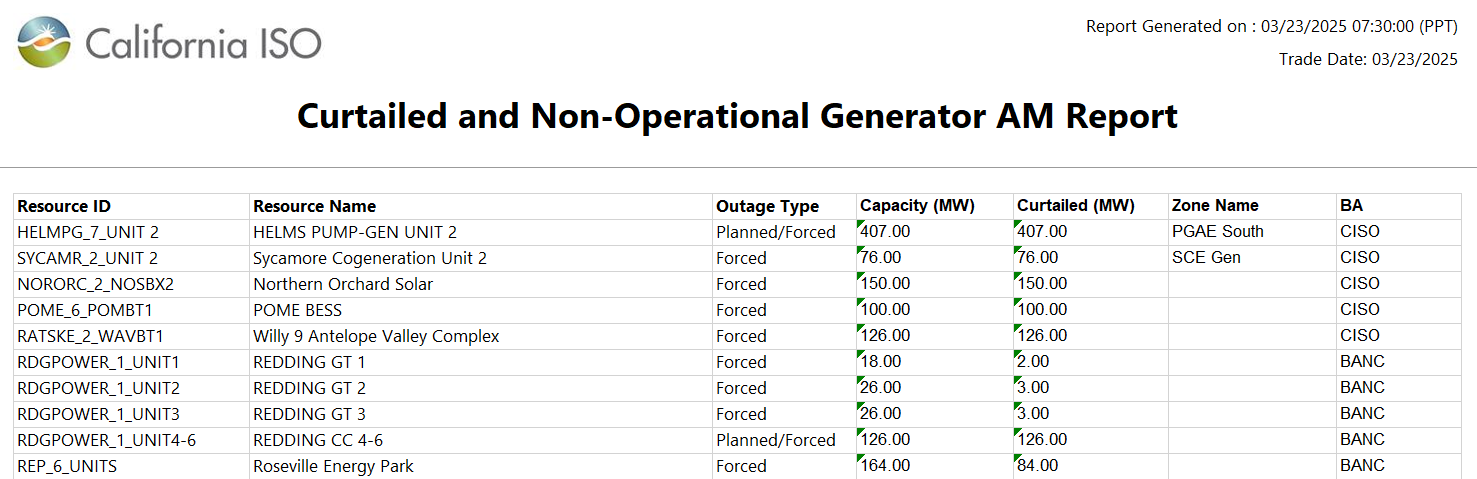
\includegraphics[scale=0.40]{graphic/caiso-snippet.png}}
\caption{An example of a publicly-posted dataset from CAISO}
\label{fig:caiso-outage-example}
\end{figure}

Such a dataset enables this system to perform surveillance and analysis on generators in a market to screen for physical withholding, or other market gaming schemes. For further information on where to view live data from these systems, see Appendix \ref{appendix:E} for a full reference of the systems that currently exist as public sources of market data. 

\section{Information Architecture and Domain-Specific Languages}

\subsection{The Importance of Institutional Knowledge}

Another area that this research intends to address is maintaining institutional knowledge. As employees retire or make career changes into other industries, the institutional knowledge that they built often leaves with them. In market monitoring, this problem is amplified due to two, salient facts: 1) the number of individuals that work in market monitoring are small compared to the rest of the energy and utilities industries, and 2) market monitors often specialize in regards to analysis or policy work. Individuals who primarily work in market surveillance may never directly work in policy development for generator capacity accreditation.

In a personal anecdote, this "brain drain" has been seen within the SPP MMU. Several long-term employees have exited the MMU in pursuit of other roles, only to leave undocumented code behind them that others must support. This code exists in the form of SQL queries and/or SAS scripts that contain embedded business rules (as they were understood by these employees). Deciphering and supporting this code becomes a burden for others that inherit the work of these departed employees.

A 2016 publication \textit{Knowledge Management in Esoteric Management} summarizes this issue well: "...knowledge sharing should be encouraged by placing employees working together closely to create pooled expertise..." \cite{knowledge-management-in-esoteric-management}. When employees share knowledge, they can keep important information from being destroyed when key individuals leave a department. A system described this dissertation aims to foster knowledge sharing amongst employees.

\subsection{Metadata Curation}

To make sense of market monitoring data and develop an effective analytics prototype to aid market monitors in their work- understanding and mapping the metadata that governs the processes and workflows of market monitors is paramount. A recent study, \textit{Research on Power Market Data Asset Management Framework}, identifies the use of a Data Management Capability Maturity Assessment Model (DCMM) that aids in data cataloging and metadata curation for the power systems industry. Their methodology takes a holistic view of analyzing how data and metadata are used in market contexts, and creates a topology system for cataloging such data \cite{marketdataasset}.

\subsection{Domain-Specific Languages}

Domain-specific Languages (DSL) are powerful interfaces that enable subject-matter experts (SME) in any particular domain of expertise to perform tasks similar to a proper software developer that builds applications in general-purpose languages (GPL). A well-defined DSL can save many man-hours in development time for specific groups that have IT oriented needs, but lack the funding or access to talent for hiring a normal software engineer. DSLs also have the ability to lower the “barriers to entry” for SMEs that wish to write applications to handle work within their purview. With support from a DSL- a software engineer does not need to be deeply involved in business rules to understand how to develop an application (a common issue in the energy industry). Likewise, SMEs do not need to heavily codify their business rules into software requirements for an application to be developed.

The literature uncovered in this review supports both the claim that DSLs have high efficacy in financial contexts. Krasts, Kleins, and Teilans (2012) illustrates how domain-specific languages have been used in modeling the complex dynamics of financial settlements systems \cite{krasts}. Additionally, the literature shows that DSLs have been deployed in other areas of the energy sector, as identified by Sobernig, Strembeck, and Beck \cite {beck} in \textit{Developing a Domain Specific Language for Scheduling in the European Energy Sector}. While this paper sets precedent for the use of DSLs in the energy industry, it presents an even larger gap that this dissertation intends to address. Beck’s study only explores tagging and scheduling, which only encompasses a single component of market monitoring. Additionally, and far more importantly, the implementation of their DSL was constrained to a specific market interconnection in Europe, which is significantly less complex than the transmission and congestion \footnote{Current issues in North America show large pockets of stranded load, which have significant economic (and, by extension, reliability) implications. Congestion on the BES constitutes a market (Financial Transmission Rights) that settles for billions of dollars. This is all due to the fact that monies have to be paid to rights holders for transmitting energy across a congested transmission infrastructure.} issues that are seen throughout the North American Bulk Electric System.

The software industry has, similarly, invested in making domain-specific languages more accessible to business users. Jetbrains (a prominent vendor in the developer tooling and integrated development environment space) has developed a workbench application- MPS (Meta-Programming System), a “projectional editor”- to allow non-developers to create DSL-like applications for business purposes. “Domain experts with inclination towards programming but without formal education in computer science will themselves build or customize DSLs to address the needs specific in their domains” \cite{ratiu}. The experience that Jetbrains developers have with educating others in the use of MPS support this idea.

Another area of DSLs that is essential to a successful implementation in market monitoring is modeling. Modeling, like in other areas of business and engineering, is how business rules are effectively mapped to artifacts in software engineering \cite{lethrech}. Modeling market monitoring concepts effectively is a critical step in ensuring that the system meets the needs of analysts and business users.

\section{Research Design and Contributions}

This project's design is based on the Design Science Research Methodology (DSRM), a process for developing new product artifacts. The researcher chose the DSRM for this project because the main research objective is to develop a domain-specific language for market monitors to use in their analysis.

Data and information quality problems exist today in the market monitoring body of knowledge. Domain-specific languages are powerful models for allowing users to systematically solve problems within a specific domain. As was determined in the literature review, DSLs have only had limited exposure in electricity markets (and even less exposure in market monitoring). This discovered gap in existing research serves as the inspiration for this project. Figure \ref{fig:dsrm-diagram} provides more detail on the planned use of design science within this project. \footnote{See Appendix \ref{appendix:C} for a schedule of the milestones and expected completion timeline for this project.}

\begin{figure}[ht]
\centering
\fbox{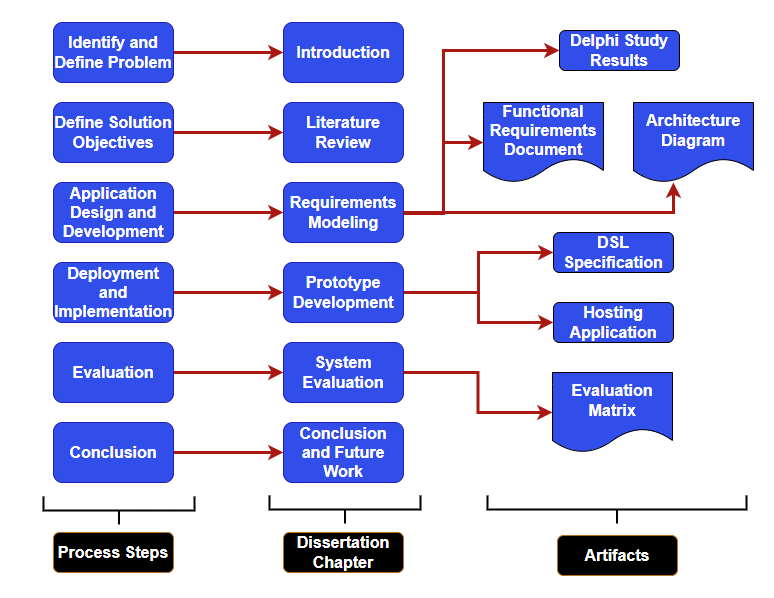
\includegraphics[scale=0.65]{graphic/dsrm-revised-diagram.png}}
\caption{Design Science Research Methodology for this dissertation}
\label{fig:dsrm-diagram}
\end{figure}

As established by the literature review, this project is a unique research endeavor in the following objective areas:

\begin{itemize}
    \item{It aims to develop a novel, interactive development environment for performing market surveillance and analysis}
    \item{It shall advance the field of information quality by providing a foundation (by way of a systematic literature review) for what information quality research has been conducted in the market monitoring domain, and what future opportunities exist}
    \item{It shall provide a flexible, metadata-driven architecture design that allows market monitors to fetch data from a variety of sources and formats that are used in market monitoring investigations. This design will be determined through use of the Delphi methodology}
    \item{It shall perform an evaluation of the proof-of-concept prototype system for determining to what degree the system satisfies the requirements gathered in the Delphi study \footnote{This component of the research evaluates how well the current needs of market monitors are met. This has importance to the industry because, while market monitors are supplied with data from their jurisdictional markets, MMUs often must provide their own in-house support for programming and surveillance. The system described in this research gives way to a common, open-source, platform that market monitors can develop and extend for their own work.}}
\end{itemize}

In addition to a domain-specific language for analyzing electricity market data, the system implementation portion of this project will also include a web application (with tooling) that showcases the language's ability to aid in producing information products for MMUs.

\subsection{Proposed Investigation}

The investigation design for this dissertation is composed of 5 main components: a literature review, requirements gathering from subject matter experts, an architecture design (and accompanying documentation), development of a prototype that serves as an example implementation of the architecture design, and a period of evaluation to determine to what degree the prototype system satisfies the requirements document.

\subsection{Limitations of This Research}

The scope of work proposed in this dissertation is limited to the objectives outlined in the Research Contributions section. Specifically, it shall evaluate the artifact output of the DSRM process to ensure that the artifact functions as a “minimum viable product” for energy market analysis.

The proof-of-concept prototype discussed in this dissertation is not intended to be a production-ready system. It is not expected to be used in a live scenario for market monitors to immediately put into service. The data ingested into the prototype will be based on realistic data scraped from public data systems shown in Appendix \ref{appendix:E}. The evaluation of this system will be based upon a requirements matrix developed from the results of the Delphi study that is also conducted in this research.

Further system optimization, bug-fixes, scalability, and use in live market monitoring scenarios are all considered "out of scope" for this dissertation, and are reserved for future work.

\subsection{Analysis of Domain-Specific Languages}

If one considers programming languages as a spectrum, one such valid model could place General Purpose Languages (GPL) at one end of the spectrum and Domain-Specific Languages (DSL) on the opposite end. DSLs are languages that are limited in purpose, scope, and grammar. Rather than supporting a programming language that can be utilized for constructing, theoretically, anything- DSLs are created to solve problems that are bound to a single problem domain.

\subsubsection{Prominent Domain-Specific Languages}

\begin{table}[ht]
    \centering
        \begin{tabular}{|p{6cm}|p{4cm}|p{4cm}|p{2cm}|}
        \hline
        \textbf{Language} & \textbf{Supporting \newline Enterprise} & \textbf{Problem Domain} & \textbf{Paradigm} \\
        \hline
        Structured Query Language (SQL) & Various & Data Retrieval & Declarative \\
        \hline
        Terraform / HCL & Hashicorp & Cloud Infrastructure Deployment & Declarative \\
        \hline
        awk & Bell Labs (originally) & Text Processing & Procedural \\
        \hline
        Apache Pig ("Pig Latin") & Yahoo & Data Retrieval \newline \& Processing & Declarative \\
        \hline
        \end{tabular}
    \caption{Selection of Well-Known Domain-Specific Languages}
    \label{tab:well-known-dsl}
\end{table}

Structured Query Language (SQL) is one such example of a DSL. SQL queries are designed to retrieve data from databases for extraction, reference, and analysis. SQL dialects have been designed to interface across a broad range of database management systems (for example: PL/SQL for Oracle or T-SQL for Microsoft SQL Server).

Terraform (HCL), a product of Hashicorp Corporation, is yet another example of a domain-specific language that is prevalent among cloud-based companies. Terraform is known as an "infrastructure-as-code" language, used to interact with numerous cloud platform providers (e.g. Amazon Web Services) to quickly deploy, scale, and spin-down cloud resources. Instead of requiring an engineer to use a console environment to configure cloud resources, that same engineer can write a set of scripts that will precisely configure and deploy all of their desired infrastructure at once.

Apache Pig (and its associated programming language - Pig Latin) is also a DSL variant. Like SQL, it is a declarative language used for data retrieval and data processing. Developers at Yahoo created Pig as a way to abstract some of the complexity of SQL away from analysts that were working with large datasets. With fewer lines of code, an analyst could use Pig to parse and load a dataset into memory, perform processing tasks, and format and report the results. This was specifically useful to analysts processing large datasets because Pig also took advantage of the high-performance computing facilities of Hadoop.

Yet another powerful example of DSLs can be seen in the ubiquitous Unix program: awk. Originally created by Unix developers Aho, Weinberger, and Kerninghan, awk is a scripting language designed to process textual data- one line ata time. The power of this system allows individuals to write expressions that are 1) simple to understand, 2) efficient, and 3) portable across different Linux implementations. Countless developers (including the researcher of this dissertation) have made use of awk's utilities to process and format data in a headless environment.

Each of the languages represented in this review are, on their own, infeasible for writing general purpose applications. SQL, for example, should not be used to write a desktop program. They were, instead, each created to solve specific issues within their respective problem domains. Likewise, Terraform cannot be used to create web applications or develop billing software. One of the "upsides" of these languages are that they can quickly handle tasks within a specific problem domain. 

\subsubsection{DSL Variations}

\subsubsection{Application to Market Monitoring Research}